% !TeX program = pdflatex
\documentclass[tikz,border=8pt]{standalone}
\usepackage{tikz}
\usetikzlibrary{calc,angles,quotes,positioning}
\definecolor{FigureBlue}{HTML}{2563EB}
\definecolor{FigureOrange}{HTML}{EA580C}
\begin{document}
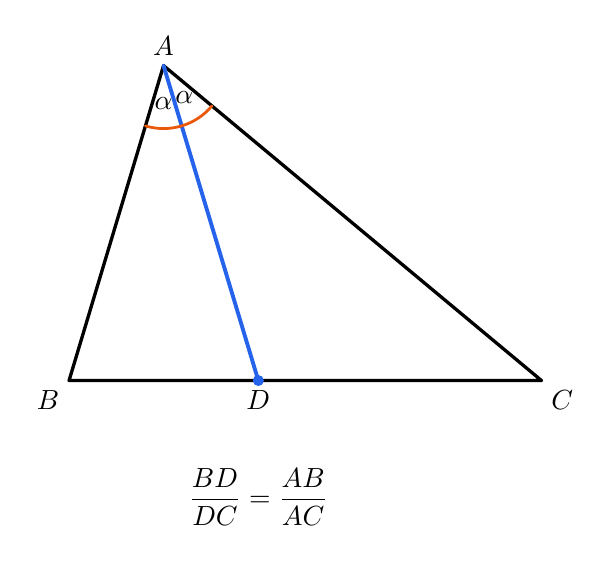
\begin{tikzpicture}[line cap=round,line join=round]
  \coordinate (A) at (1.2,4);
  \coordinate (B) at (0,0);
  \coordinate (C) at (6,0);
  \pgfmathsetmacro{\AB}{veclen(1.2,4)}
  \pgfmathsetmacro{\AC}{veclen(4.8,4)}
  \pgfmathsetmacro{\ratio}{\AB/(\AB+\AC)}
  \coordinate (D) at ($(B)!\ratio!(C)$);
  \draw[line width=1.2pt] (A)--(B)--(C)--cycle;
  \draw[FigureBlue,line width=1.4pt] (A)--(D);
  \pic[draw=FigureOrange,line width=1pt,angle radius=8mm,"$\alpha$"] {angle=B--A--D};
  \pic[draw=FigureOrange,line width=1pt,angle radius=8mm,"$\alpha$"] {angle=D--A--C};
  \fill[FigureBlue] (D) circle (2pt);
  \node[above] at (A) {$A$};
  \node[below left] at (B) {$B$};
  \node[below right] at (C) {$C$};
  \node[below] at (D) {$D$};
  \node[below=10mm of D] {$\displaystyle\frac{BD}{DC}=\frac{AB}{AC}$};
\end{tikzpicture}
\end{document}
